\begin{Exercise}[label = cristall, title = Relexion im Kristall, difficulty = 3, origin = Aaron Wild]
	Betrachte einen Kristall der Länge $\ell$ und Höhe $1$ (in der gleichen Einheit wie $\ell$), in dem aus irgendeinem Grund Licht der Leistung $P$ entsteht.\\
	\Question
	Jedes Mal, wenn das Licht die äußere Wand trifft, wird ein Anteil $R$ der Leistung reflektiert, und ein Teil $(1-R)$ der Leistung verlässt den Kristall. Wie groß ist die Leistung $p$, die den Kristall auf der anderen Seite verlässt?
	\Question Beschreibe die selbe Situation für den Fall, dass das Licht sich nicht parallel zur Kante des Kristalls ausbreitet, sondern unter einem Winkel $\theta$.

\end{Exercise}
\begin{figure}[h]
	\centering
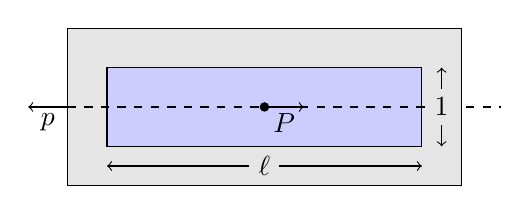
\begin{tikzpicture}
\filldraw[fill=gray!20!white, draw=black] (-.5,0) rectangle (4.5,2);
\filldraw[fill=blue!20!white, draw=black] (0,.5) rectangle (4,1.5);
\filldraw[black] (2,1) circle (1.5pt);
\node at (2.25,0.8) {$P$};
\draw[->] (2,1) -- (2.5,1);
\draw[dashed] (-.5,1) -- (5,1);
\draw[->] (-.5,1) -- (-1,1);
\node at (-.75,0.8) {$p$};
\draw[<->] (0,.25) to node[midway, fill = gray!20!white]{$\ell$} (4,.25);
\draw[<->] (4.25,.5) to node[midway, fill = gray!20!white]{$1$} (4.25,1.5);
\end{tikzpicture}
\end{figure}
